\section{Control}

\begin{figure}[h]
	\centering
	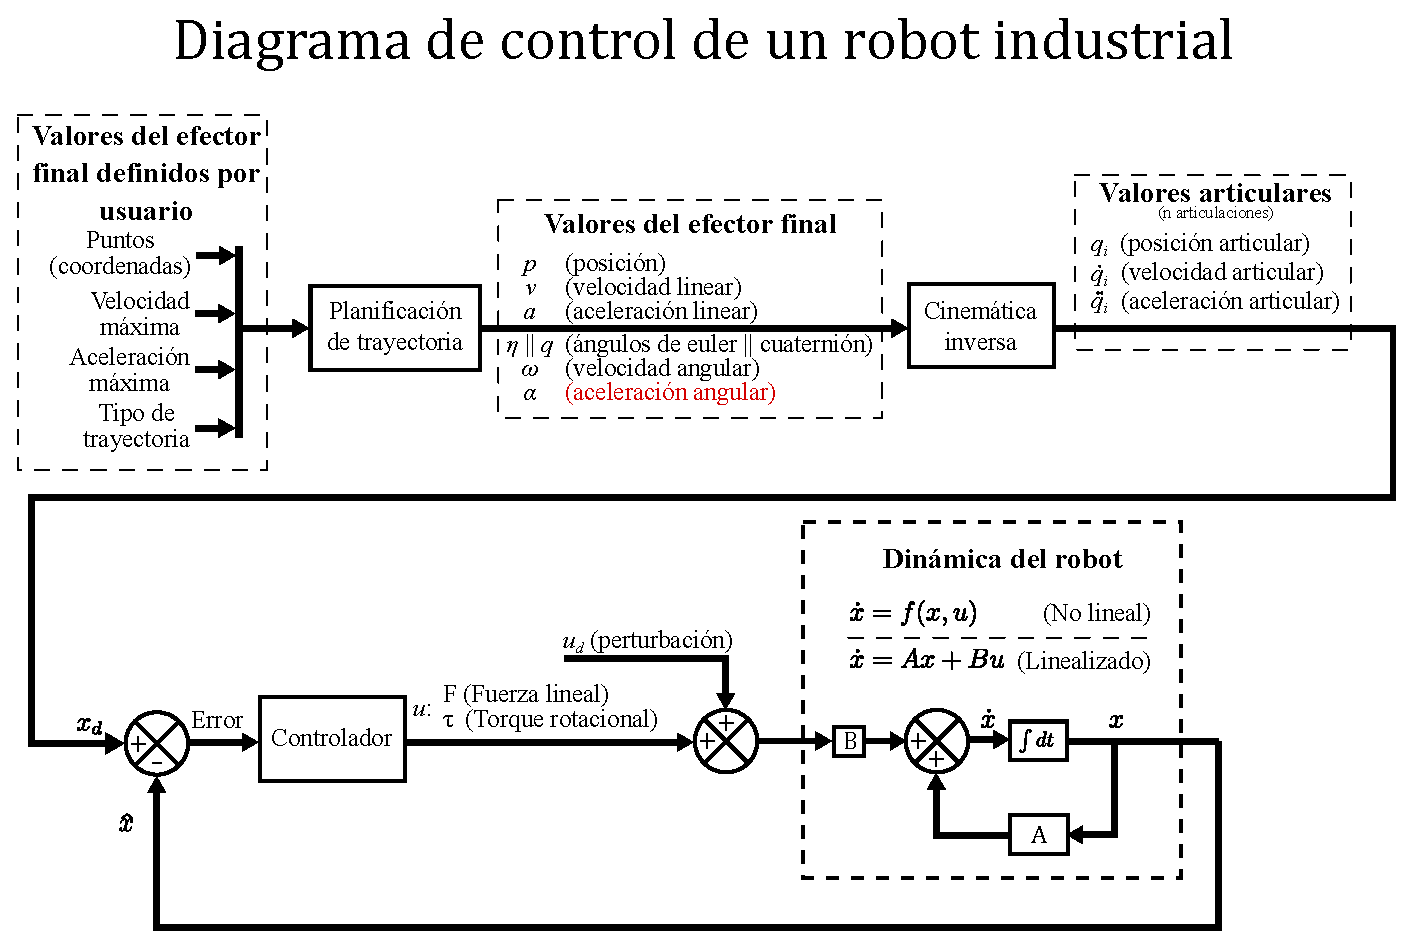
\includegraphics[width=\linewidth]{img/Diagrama_robot_industrial}
	\caption{Diagrama de bloques de un robot industrial}
	\label{fig:diagrama-de-robot-industrial}
\end{figure}

\subsection{Explicación del Diagrama de Control de un Robot Industrial}

La \autoref{fig:diagrama-de-robot-industrial}. muestra el diagrama de bloques de un sistema de control para un robot industrial. A continuación se explica paso a paso cómo funciona este sistema, de una forma clara y sencilla.

\subsubsection{1. El usuario da los objetivos}

Todo empieza cuando el usuario le indica al robot lo que debe hacer. Por ejemplo:
\begin{itemize}
	\item Las coordenadas del punto al que debe llegar el efector final.
	\item La velocidad y aceleración máximas permitidas.
	\item El tipo de trayectoria (recta, curva, interpolada, etc.).
\end{itemize}

\subsubsection{2. Planificación de trayectoria}

Con esa información, el sistema genera una trayectoria continua para el efector final. Es decir, calcula cómo debería moverse el efector en el espacio con respecto al tiempo. Se obtienen:
\begin{itemize}
	\item Posición \( \mathbf{p} \)
	\item Velocidad lineal \( \mathbf{v} \)
	\item Aceleración lineal \( \mathbf{a} \)
	\item Orientación \( \theta \) (ángulos de Euler o cuaterniones)
	\item Velocidad angular \( \boldsymbol{\omega} \)
	\item Aceleración angular \( \boldsymbol{\alpha} \)
\end{itemize}

\subsubsection{3. Cinemática inversa}

Después, se usa la cinemática inversa para convertir la trayectoria en el espacio cartesiano a valores que el robot pueda usar: posiciones, velocidades y aceleraciones en las articulaciones:
\[
\mathbf{q}, \quad \dot{\mathbf{q}}, \quad \ddot{\mathbf{q}}
\]

\subsubsection{4. Controlador}

Aquí entra el controlador. Lo que hace es comparar el estado deseado del robot con el estado real (medido con sensores o estimado). Esa diferencia se llama \textbf{error}.

Con ese error, el controlador calcula las señales de control \( \mathbf{u} \), que pueden ser fuerzas o torques, para mover las articulaciones del robot.

\subsubsection{5. Dinámica del robot}

El robot responde a esas señales de control mediante su modelo dinámico, que predice cómo se moverá según las fuerzas aplicadas. Esto puede modelarse de forma:
\begin{itemize}
	\item \textbf{No lineal:} \( \dot{\mathbf{x}} = f(\mathbf{x}, \mathbf{u}) \)
	\item \textbf{Linealizada:} \( \dot{\mathbf{x}} = A\mathbf{x} + B\mathbf{u} \)
\end{itemize}

También se puede incluir una perturbación externa \( \mathbf{u}_d \), como una fuerza inesperada o un error en el modelo.

\subsubsection{6. Ciclo cerrado (retroalimentación)}

Después de aplicar el control y que el robot se mueve, se mide su estado nuevamente y se vuelve a enviar al controlador. Así se forma un \textbf{lazo cerrado}, que corrige constantemente el movimiento del robot en tiempo real.

\subsubsection{Resumen}

Este diagrama representa el flujo completo de control de un robot industrial:
\begin{enumerate}
	\item Se definen los objetivos.
	\item Se genera una trayectoria.
	\item Se calcula cómo mover las articulaciones.
	\item Se controlan los motores.
	\item El robot se mueve según su dinámica.
	\item Y se repite el ciclo para corregir errores.
\end{enumerate}

Todo esto permite que el robot se mueva con precisión, incluso si hay perturbaciones o cambios inesperados.
